\documentclass[aspectratio=169]{beamer}

\makeatletter
\appto\input@path{{pkgs/awesome-beamer},{pkgs/smile}}
\makeatother
\graphicspath{{meta/title_pic}}

\definecolor{c}{HTML}{6a393b}
\usetheme[english,notoc,color,coloraccent=c,tikz,listings,htmlunderline]{awesome}

\usepackage[sfdefault]{FiraSans}
\usepackage{fontawesome5}
\usepackage{emoji}
\usepackage{tikzpingus}

\usepackage[backend=biber,style=numeric,sorting=none,sortcites=true]{biblatex}
\usepackage[strict,autostyle]{csquotes}
\addbibresource{refs.bib}

\def\footcite#1{%
	\begingroup%
	\renewcommand\thefootnote{}%
	\cite{#1}%
	\footnotetext{\cite{#1}~\fullcite{#1}}%
	\addtocounter{footnote}{-1}%
	\endgroup%
}

\usepackage[duration=20,defaulttransition=fade,enduserslide=13]{pdfpc}
\newcommand<>{\talknote}[1]{\only#2{\pdfpcnote{- #1}\relax}}

\background{main.pdf}
\title{Slicing Coverage}
\subtitle{Towards improved code coverage metrics}
\author{Lukas Pietzschmann}
\email{lukas.pietzschmann@uni-ulm.de}
\institute{Institute of Software Engineering and Programming Languages}
\uni{Ulm University}
\location{Ulm}
\date{November 5\textsuperscript{th}, 2024}

\def\flowr{\emph{flowr}}
\def\covr{\emph{covr}}
\def\ergo{\raisebox{-1pt}{\faAngleRight}}
\makeatletter
\newcommand\ghuser[2][2.5mm]{\begin{tikzpicture}\tikzset{c/.style={roundnode,inner sep=0,outer sep=0,##1}}
	\node[c=black,minimum width=#1+\smile@linewidth,shadow] at (0,0) {};
	\clip (0,0) circle (#1/2);
	\node at (0,0) {\includegraphics[width=#1]{#2.jpeg}};
\end{tikzpicture}}\makeatother

\usetikzlibrary{shadings,fadings,patterns,decorations.markings}
\tikzfading[name=fade in,inner color=transparent!100,outer color=transparent!0]
\tikzfading[name=fade out,inner color=transparent!0,outer color=transparent!100]
\tikzfading[name=ffade out, inner color=transparent!64, outer color=transparent!100]
\tikzset{
	line/.style={roundednode,fill=gray,draw=gray,minimum height=2mm,minimum width=#1mm,anchor=west},
	cov/.style={fill=red!10!gray,draw=red!10!gray},
	slc/.style={draw=red!30!darkgray},
	pipelinestep/.style={lw,rnd,shape=signal,signal from=west,signal pointer angle=130,minimum width=3cm,minimum height=2cm,draw=black,fill=lightgray!50!white},
	ffill/.style n args={2}{path picture={
		\fill[#1] (path picture bounding box.south west) rectangle ($(path picture bounding box.north west)!#2!(path picture bounding box.north east)$);
	}}
}
\pgfkeys{/pgf/decoration/.cd,
	width factor/.store in =\wfactor,
	start color/.store in =\startcolor,
	end color/.store in =\endcolor
}
\makeatletter
\pgfdeclaredecoration{width and color change}{initial}{%
	\state{initial}[width=0pt, next state=line, persistent precomputation={%
		\pgfmathdivide{50}{\pgfdecoratedpathlength}%
		\let\increment=\pgfmathresult%
		\def\x{0}%
	}]{}
	\state{line}[width=.5pt, persistent postcomputation={%
		\pgfmathadd@{\x}{\increment}%
		\let\x=\pgfmathresult%
	}]{%
		\pgfsetlinewidth{\wfactor*\x/50*0.075pt+\pgflinewidth}%
		\pgfsetarrows{-}%
		\pgfpathmoveto{\pgfpointorigin}%
		\pgfpathlineto{\pgfqpoint{.75pt}{0pt}}%
		\pgfsetstrokecolor{\endcolor!\x!\startcolor}%
		\pgfusepath{stroke}%
	}
	\state{final}{%
		\pgfsetlinewidth{\pgflinewidth}%
		\pgfpathmoveto{\pgfpointorigin}%
		\color{\endcolor!\x!\startcolor}%
		\pgfusepath{stroke}%
	}
}
\makeatother
\xdefinecolor{LightY}{RGB}{247, 225, 34}
\lstset{tabsize=2,texcl=false}
\lstdefinelanguage{json}{
	literate=
		{:}{{{\color{darkgray}{:}}}}{1}
		{,}{{{\color{darkgray}{,}}}}{1}
		{\{}{{{\color{darkgray}{\{}}}}{1}
		{\}}{{{\color{darkgray}{\}}}}}{1}
		{[}{{{\color{darkgray}{[}}}}{1}
		{]}{{{\color{darkgray}{]}}}}{1},
}
\lstdefinelanguage{myr}{
	keywords={function,return,if,else,library},
	otherkeywords={!,!=,~,*,\&,\%/\%,\%*\%,\%\%,<-,<,<=,+,-,/},
	alsoother={._$},
	sensitive,
	morecomment=[l]\#,
	morestring=[d]",
	morestring=[d]'
}
\newcommand\ri[2][]{\lstinline[language=myr,#1]{#2}}

\begin{document}

\maketitle

\section{Motivation}
\newsavebox\fibcode
\newsavebox\fibtest
\begin{lrbox}{\fibcode}\begin{lstlisting}[language=myr]
	invocations <- 0
	fib <- function(n) {
		invocations <<- invocations + 1
		if (n <= 1)
			return(n)
		else
			return(fib(n - 1) + fib(n - 2))
	}
\end{lstlisting}\end{lrbox}
\begin{lrbox}{\fibtest}\begin{lstlisting}[language=myr]
	library(testthat)

	test_that("fib works", {
		expect_equal(fib(6), 8)
	})
\end{lstlisting}\end{lrbox}
\begin{frame}[fragile]
	\frametitle{What's wrong with coverage?}
	\usebox\fibcode\par\medskip
	\begin{itemize}[<+(1)->]
		\item Typical implementation of the Fibonacci function
		\item But as a side effect, we also count the number of invocations
	\end{itemize}
\end{frame}

\begin{frame}[fragile]
	\frametitle{What's wrong with coverage?}
	\usebox\fibtest\par\medskip
	\begin{itemize}
		\item<2-> We can calculate the test's coverage like the following:
	\end{itemize}
	\begin{visibleenv}<3->
	\begin{lstlisting}[language=myr]
		> covr::file_coverage("fib.R", "test.R")
		Coverage: 100.00%
		fib.R: 100.00%
	\end{lstlisting}
	\end{visibleenv}
	\begin{itemize}[<+(3)->]
		\item The test succeeded and while we did achieve full coverage, the test didn't validate every behavior
		\item The correct value of \ri{invocations} was never checked
	\end{itemize}
\end{frame}

\def\fade#1#2{\draw[fill=white,draw=none,path fading=#1] (#2.north west) rectangle (#2.south east);}
\def\sparklecnt{200}
\def\outerradius{15mm}
\newsavebox\sparkle
\newsavebox\sparklefield
\newsavebox\rays
\savebox\sparkle{\begin{tikzpicture}[scale=0.02]
	\draw[line join=round,draw=yellow!50!black,fill=yellow] (0,5) .. controls(0.2,1) .. (10,0) ..controls (0.2,-1) ..(0,-5).. controls(-0.2,-1)..(-10,0) .. controls(-0.2,1).. cycle;
\end{tikzpicture}}
\savebox\sparklefield{\begin{tikzpicture}
	\pgfmathsetmacro {\goldenRatio} {(1+sqrt(5))}
	\foreach \b in {1,...,\sparklecnt}{
		\pgfmathsetmacro{\angle}{mod(\goldenRatio * \b,2)*180}
		\pgfmathsetmacro{\sradius}{\b / \sparklecnt * \outerradius / 10}
		\node at (\angle:\sradius) {\usebox\sparkle};
	}
	\fade{fade in}{current bounding box}
\end{tikzpicture}}
\savebox\rays{\begin{tikzpicture}
	% small fading rays
	\foreach \a in {0, 60, ..., 300}{%
		\draw[decoration={
			width and color change,
			width factor=.1,
			start color=red!50!yellow,
			end color=yellow!40!white
		}, decorate] (\a+30: 3.5) -- (0, 0);
	}

	% long rays
	\foreach \a in {0, 60, ..., 300}{%
		\draw[decoration={
			width and color change,
			width factor=.3,
			start color=red!50!yellow,
			end color=yellow
		}, decorate] (\a+5: 5) -- (0, 0);
	}
	\foreach \a in {0, 60, ..., 300}{%
		\draw[decoration={
			width and color change,
			width factor=.1,
			start color=red!50!yellow,
			end color=yellow
		}, decorate] (\a+5: 5) -- (0, 0);
	}

	% higlights
	\fill[LightY!20!white, path fading=fade out] (0, 0) circle (.8);
	\foreach \a in {0, 60, 120}{%
		\fill[yellow!50!white, path fading=ffade out, rotate={\a+5}]
		(0, 0) ellipse [x radius=1.3, y radius=1];
	}
\end{tikzpicture}}
\begin{frame}[fragile]
	\frametitle{What's wrong with coverage?}
	\begin{itemize}[<+(1)->]
		\item The coverage score needs to account for what is actually checked by a test
		\item Therefore we propose:
	\end{itemize}\par\medskip
	\begin{visibleenv}<6->
	\begin{block}[\emph{Slicing Coverage}]
		A novel way of calculating coverage that considers what is actually checked by the test.
	\end{block}
	\end{visibleenv}
	\begin{onlyenv}<4>
	\begin{tikzpicture}[o]
		\draw[fill=white,draw=white] (current page.north west) rectangle (current page.south east);
		\node[] at (current page) {\usebox\sparklefield};
		\node[] at (current page) {\usebox\rays};
		\node[text width=1.6cm,align=center,node on layer=foreground,scale=2] (slc) at (current page) {\contour{white}{Slicing}\\\contour{white}{Coverage}};
		\node[fit=(slc),inner sep=1cm] (F) {};
		\fade{fade out}{F}
	\end{tikzpicture}
	\end{onlyenv}
\end{frame}

\begin{frame}
	\frametitle{Shortcomings of slicing coverage}
	We have to distinguish between two kinds of shortcomings:
	\begin{columns}[c]
		\begin{column}<2->{0.45\textwidth}
			\begin{block}[Implementation related]
				Implicit assumptions that are not expressed through code
			\end{block}
		\end{column}
		\begin{column}<3->{0.45\textwidth}
			\begin{block}[Conceptual]
				The results quality is dependent on the quality of the slice
			\end{block}
		\end{column}
	\end{columns}\par\bigskip
	\onslide<4->{While we can solve implementations shortcomings, conceptual shortcomings are inherent to slicing coverage.}
\end{frame}

\section{Related Work}
\begin{frame}
	\frametitle[Fault Localization]{Related Work}
	% \begin{block}[Key Takeaways]
		\begin{itemize}[<+(1)->]
			\item Not all covered code contributes to the test's outcome~\footcite{soha2023}
			\item Dynamic slicing can be used to identify statements containing faulty code~\footcite{zhang2005}
			\item \citeauthor{reis2019} measured an increase in accuracy of fault localization by up to 73.7\%~\footcite{reis2019}
		\end{itemize}\par\bigskip
	% \end{block}\par\bigskip
	\onslide<5->{While slicing coverage does not localize faults, it does aim to improve coverage based values using slicing.}
\end{frame}

\tikzset{paper/.style={roundednode,anchor=south east,rotate=#1,shadow}}
\newsavebox\paper
\savebox\paper{\begin{tikzpicture}
	\node[paper=-10,xshift=4mm] (3) {\includegraphics[page=3,width=2.5cm]{assets/checkedcov.pdf}};
	\node[paper=-05,xshift=2mm] (2) {\includegraphics[page=2,width=2.5cm]{assets/checkedcov.pdf}};
	\node[paper=-00,xshift=0mm] (1) {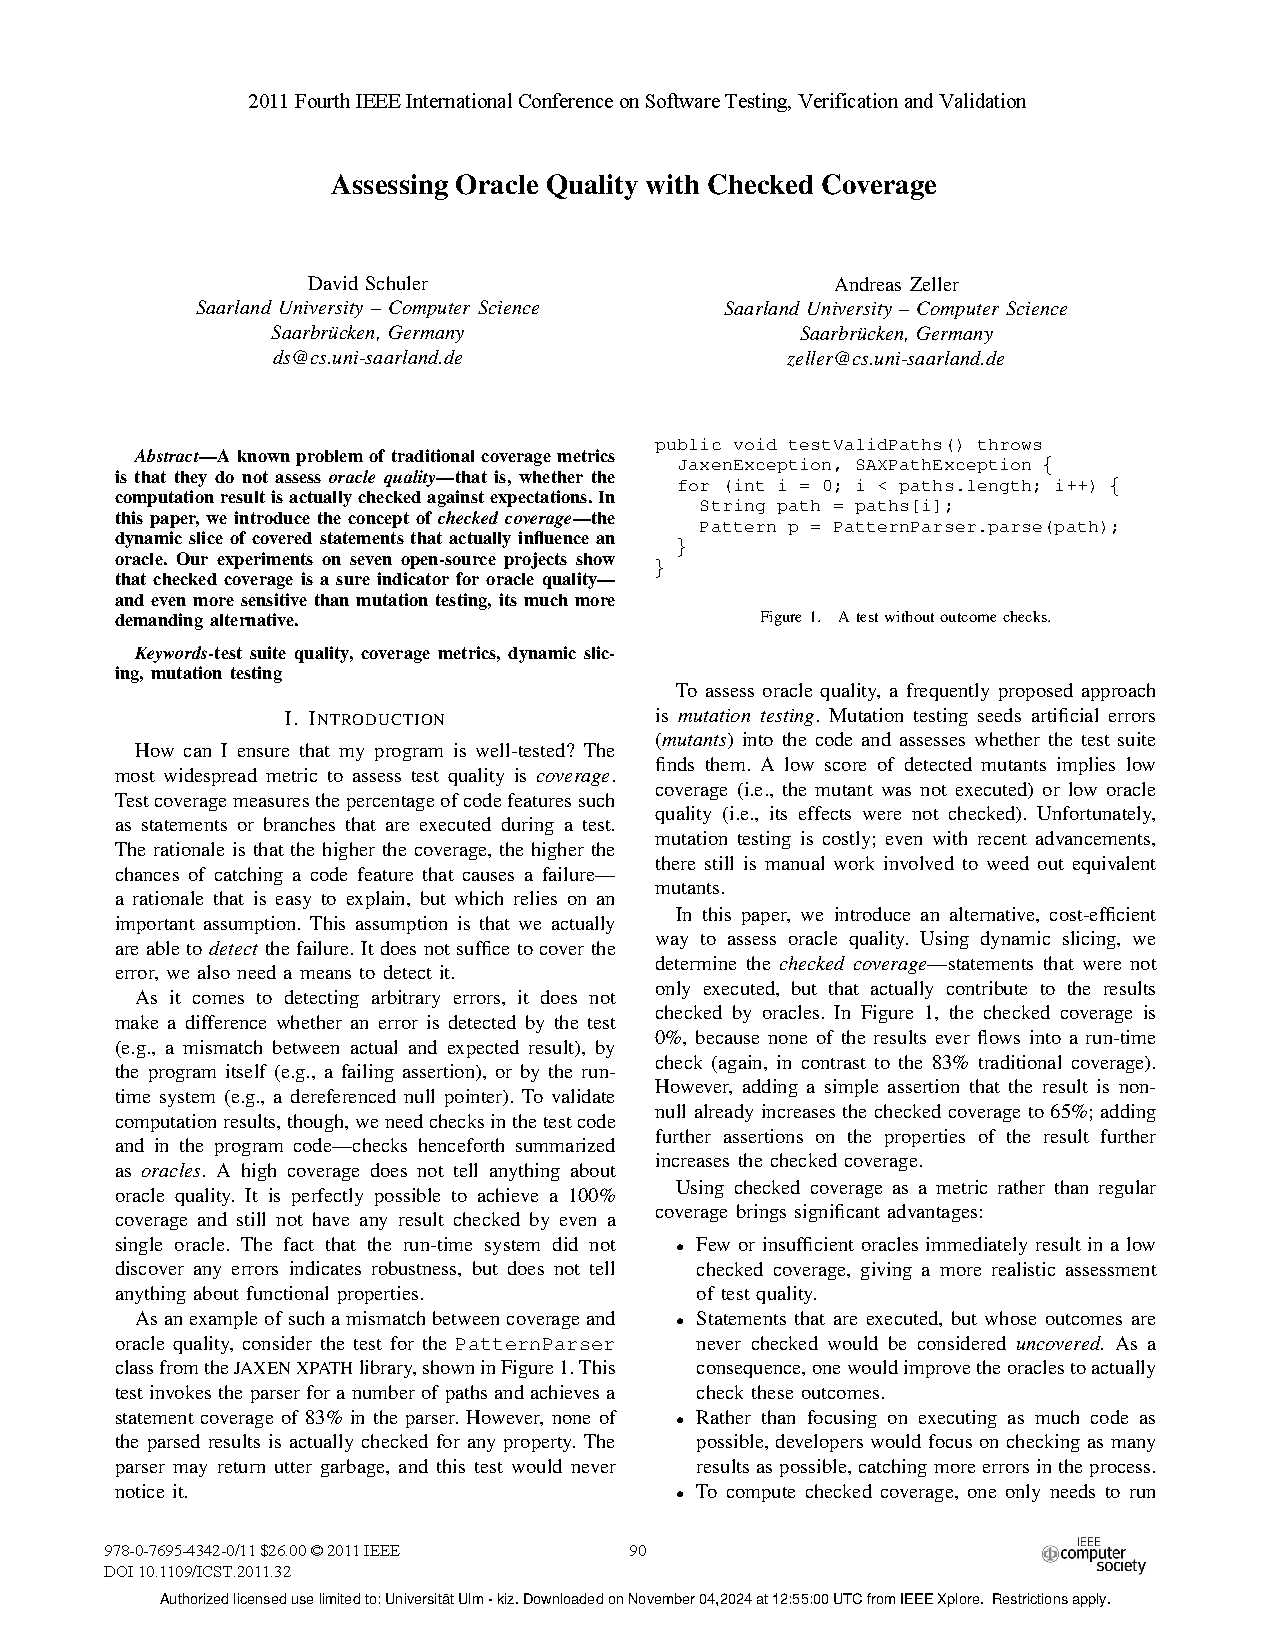
\includegraphics[page=1,width=2.5cm]{assets/checkedcov.pdf}};
\end{tikzpicture}}
\begin{frame}
	\frametitle[Checked Coverage]{Related Work}
	\begin{wide}
	\begin{columns}[c]
		\begin{column}<2->{\dimexpr\textwidth-\wd\paper\relax}
			{\large\bfseries We're not the first ones to think about this!}\par\bigskip
			\begin{itemize}
				\item<3-> \citeauthor{schuler2011} introduced the concept of checked coverage in \citeyear{schuler2011}~\footcite{schuler2011}
				\item<4-> They use dynamic slicing to determine the  proportion of executed statements that contribute to values verified by the test
			\end{itemize}
		\end{column}
		\begin{column}<3->{\wd\paper}
			\usebox\paper
		\end{column}
	\end{columns}
	\end{wide}
\end{frame}

\section{State of affairs}
\subsection{What we want to get done}

\colorlet{xx}{accent!10!lightgray}
\tikzset{rq/.style={pill,draw=accent!20!black,fill=accent!5!lightgray!50,font=\scriptsize,inner sep=2pt,shadow}}
\begin{frame}
	\frametitle{What we want to get done}
	\begin{wide}
	\begin{center}
	\begin{tikzpicture}[node distance=14mm,scale=1.5]
		\node[pipelinestep,visible on=<2->,alt={<5->{ffill={xx}{0.92}}{}},text width=2cm,align=center] (A) {Build the package};
		\node[pipelinestep,visible on=<3->,alt={<5->{ffill={xx}{0.35}}{}},text width=2cm,align=center,right=of A] (B) {Evaluate it};
		\node[pipelinestep,visible on=<4->,alt={<5->{ffill={xx}{0.20}}{}},text width=2cm,align=center,right=of B] (C) {Write about it};

		\onslide<2->{\node[rq] at (A.north east) {RQ1};}
		\onslide<3->{\node[rq,visible on=<3->] at (B.north east) {RQ2};}
	\end{tikzpicture}
	\end{center}
	\end{wide}
\end{frame}

% \begin{frame}
% 	\frametitle{Research Questions}
% 	\begin{description}[<+(1)->]
% 		\item[RQ1] How can slicing coverage be implemented for the R~programming language?
% 		\item[RQ2] In what way do the results of slicing coverage differ from those of traditional coverage?
% 			\begin{description}
% 				\item[RQ2.1] How do the results differ in terms of coverage percentage?
% 				\item[RQ2.2] Does slicing coverage actually provide more accurate results?
% 				\item[RQ2.3] How does slicing coverage affect memory and CPU usage compared to traditional coverage?
% 			\end{description}
% 	\end{description}
% \end{frame}

\subsection{What's already done}
\tikzset{
	cc/.style={alt={#1{accent,line width=1.5px}{black}}},
	sarrow/.style={arrow,short=1mm},
	arrowl/.style={pill,fill=#1,draw=none,font=\scriptsize,inner sep=.5pt},
	explainer/.style={roundednode,fill=lightgray!30,draw=gray},
	exarrow/.style={lcr,draw=gray,lw,short=1mm}
}
\newsavebox\queryb
\begin{lrbox}{\queryb}\begin{lstlisting}[language=json,style=smile@lst@plain]
{
  "type": "compound",
  "query": "call-context",
  "commonArguments": {
    "kind": "check",
    "callTargets": "global"
  },
  "arguments": [
    {
      "callName": "^expect_.*$",
      "subkind": "except"
    }
  ]
}
\end{lstlisting} \end{lrbox}
\begin{frame}
	\frametitle[Implementation]{What's already done}
	\begin{wide}\begin{center}
	\begin{tikzpicture}[node distance=1.5cm]\addtolength{\leftmargini}{-3mm}
		\onslide<2>{\node[roundednode,fill=accent,text=white,draw=accent,shadow] (core) {\bfseries Package};}
		\onslide<{1,3-}>{\node[roundednode] (core) {Package};}
		\node[roundednode,right=of core] (covr) {\covr};
		\node[roundednode,left=of core] (adap) {\flowr{} R-Adapter};
		\node[roundednode,left=of adap] (flowr) {\flowr};
		\node[roundednode,node on layer=background,dashed,lcr,inner sep=3mm,fill=lightgray!30,fit=(adap)(core)(covr)] (pkg) {};
		\node[squarenode,below=of pkg,shift={(-2cm,5mm)}] (in) {Input Files};
		\node[squarenode,below=of pkg,shift={(2cm,5mm)}] (out) {Coverage Report};

		\coordinate (M) at ($(flowr.east)!0.5!(adap.west)$);
		\draw[lightgray,dashed,lw,lcr] ([yshift=1.3cm]M) -- (in.south-|M);

		\draw[sarrow] (in)               to                node(1){} (pkg);
		\draw[sarrow] (core.north west)  to[bend right=10] node(2){} (adap.north east);
		\draw[sarrow] (adap.north west)  to[bend right=10] node(3){} (flowr.north east);
		\draw[sarrow] (flowr.south east) to[bend right=10] node(4){} (adap.south west);
		\draw[sarrow] (adap.south east)  to[bend right=10] node(5){} (core.south west);
		\draw[sarrow] (core.south east)  to[bend right=10] node(6){} (covr.south west);
		\draw[sarrow] (covr.north west)  to[bend right=10] node(7){} (core.north east);
		\draw[sarrow] (pkg)              to                node(8){} (out);

		\node[arrowl=white,visible on=<3>]           at (1) {req};
		\node[arrowl=lightgray!30,visible on=<5>]    at (2) {ana};
		\node[arrowl=white,visible on=<7>]           at (3) {ana};
		\node[arrowl=lightgray!30,visible on=<8>]    at (2) {nodes};
		\node[arrowl=white,visible on=<9>]           at (3) {nodes};
		\node[arrowl=white,visible on=<10>]          at (4) {nodes};
		\node[arrowl=lightgray!30,visible on=<11>]   at (5) {nodes};
		\node[arrowl=lightgray!30,visible on=<12-14>]at (2) {query};
		\node[arrowl=white,visible on=<15>]          at (3) {query};
		\node[arrowl=white,visible on=<16>]          at (4) {query};
		\node[arrowl=lightgray!30,visible on=<17>]   at (5) {query};
		\node[arrowl=lightgray!30,visible on=<18>]   at (2) {slice};
		\node[arrowl=white,visible on=<19>]          at (3) {slice};
		\node[arrowl=white,visible on=<20>]          at (4) {slice};
		\node[arrowl=lightgray!30,visible on=<21>]   at (5) {slice};
		\node[arrowl=lightgray!30,visible on=<22>]   at (6) {cover};
		\node[arrowl=lightgray!30,visible on=<24>]   at (7) {cover};
		\node[arrowl=white,visible on=<25>]          at (8) {res};

		% \foreach \x in {1,3,4,8}\node[circle,font=\tiny,fill=white,inner sep=.5pt] at (\x) {\x};
		% \foreach \x in {2,5,6,7}\node[circle,font=\tiny,fill=lightgray!30,inner sep=.5pt] at (\x) {\x};

		% \node[xshift=0mm] at (flowr.north west) {\ghuser{ehcsan}};
		% \node[xshift=2mm] at (flowr.north west) {\ghuser{core5563}};
		% \node[xshift=4mm] at (flowr.north west) {\ghuser{benedikt}};
		% \node[xshift=6mm] at (flowr.north west) {\ghuser{lukas}};
		% \node[xshift=8mm] at (flowr.north west) {\ghuser{julian}};
		% \node[xshift=10mm] at (flowr.north west) {\ghuser{florian}};
		%
		% \node[xshift=0mm] at (adap.north west) {\ghuser{julian}};
		% \node[xshift=2mm] at (adap.north west) {\ghuser{lukas}};
		%
		% \node[xshift=0mm] at (core.north west) {\ghuser{lukas}};

		\node[explainer,shift={(1cm,2cm)},visible on=<4->] at (core) (coree) {\scriptsize\parbox{37mm}{\begin{itemize}
			\item Provides a \covr-like API
			\item Calculates the final coverage report
		\end{itemize}}};

		\node[explainer,shift={(1.5cm,-2cm)},visible on=<23->] at (covr) (covre) {\scriptsize\parbox{25mm}{\begin{itemize}
			\item Determines covered code
		\end{itemize}}};

		\node[explainer,shift={(-1cm,2cm)},visible on=<6->] at (adap) (ae) {\scriptsize\parbox{37mm}{\begin{itemize}
			\item Hides \flowr's API behind R~functions
		\end{itemize}}};

		\draw[exarrow,visible on=<4->] (coree) -- (core);
		\draw[exarrow,visible on=<23->] (covre) -- (covr);
		\draw[exarrow,visible on=<6->] (ae) -- (adap);
	\end{tikzpicture}
	\end{center}\end{wide}
	\tikz[o]\node[yshift=7mm] at (current page.south) {\color{darkgray}\small RQ1: How can slicing coverage be implemented for the R~programming language?};
	\begin{modal}<13>[Query for exceptions]
		\usebox\queryb
	\end{modal}
\end{frame}

\begin{frame}[plain,noframenumbering]
	\begin{wide}\centering
		
\includegraphics[width=.4\textwidth]{assets/demo.png}\par
		\tiny\url{https://www.reddit.com/r/ProgrammerHumor/comments/c1n0ks/its_called_the_demo_effect/}
	\end{wide}
\end{frame}

\subsection{What still needs to be done}
\begin{frame}
	\frametitle[Evaluation]{What needs to be done}
	\begin{wide}
	\begin{center}
	\begin{tikzpicture}[node distance=1cm]
		\node[roundnode,fill=black] (S) {};
		\node[roundednode,yshift=1cm,right=of S,visible on=<2->]  (COV) {Coverage};
		\node[roundednode,yshift=0cm,right=of S,visible on=<3->]  (SLC) {Slicing coverage (static)};
		\node[roundednode,yshift=-1cm,right=of S,visible on=<4->] (MAX) {Slicing coverage (dynamic)};
		\coordinate[right=of MAX] (X);
		\node[roundnode,fill=black,visible on=<2->] at (COV -| X) (R1) {};
		\node[roundnode,fill=black,visible on=<3->] at (SLC -| X) (R2) {};
		\node[roundnode,fill=black,visible on=<4->] at (MAX -| X) (R3) {};
		\node[roundednode,fill=lightgray!30,dashed,inner sep=3mm,lcr,fit=(S)(COV)(SLC)(MAX)(R1)(R2)(R3),node on layer=background] (F) {};

		\node[squarenode,left=of F] (P) {Packages};
		\node[squarenode,right=of F] (R) {Results};

		\draw[sarrow] (P) -- (F);
		\draw[sarrow] (F) -- (R);
		\draw[sarrow,rnd,visible on=<2->] (S) |- (COV);
		\draw[sarrow,rnd,visible on=<3->] (S) |- (SLC);
		\draw[sarrow,rnd,visible on=<4->] (S) |- (MAX);
		\draw[sarrow,visible on=<2->] (COV) -- (R1);
		\draw[sarrow,visible on=<3->] (SLC) -- (R2);
		\draw[sarrow,visible on=<4->] (MAX) -- (R3);
	\end{tikzpicture}
	\end{center}
	\end{wide}
	\tikz[o]\node[yshift=7mm] at (current page.south) {\color{darkgray}\small RQ2.1: How do the results differ in terms of coverage percentage?};
\end{frame}

\begin{frame}
	\frametitle[Evaluation]{What needs to be done}
	When talking about the accuracy, we mean the following:\par\medskip
	\begin{block}[Accuracy\hfill\cite{inozemtseva2014}]
		A coverage score is considered accurate, if it correlates with the percentage of
		faults that a test is able to localize.
	\end{block}\par\medskip
	So a test yielding a score of 80\% should localize 8 out of 10 existing faults.
	\tikz[o]\node[yshift=18mm] at (current page.south) {\color{darkgray}\small RQ2.2: Does slicing coverage provide more accurate results?};
	\footnotetext{\cite{inozemtseva2014}~\fullcite{inozemtseva2014}}
\end{frame}

\begin{frame}
	\frametitle[Evaluation]{What needs to be done}
	\begin{wide}
	\begin{center}
	\begin{onlyenv}<1-4>
	\begin{tikzpicture}[node distance=1cm]
		\node[roundnode,fill=black] (S) {};
		\node[roundednode,yshift=5mm,right=of S,visible on=<2->]  (COV) {Coverage};
		\node[roundednode,yshift=-5mm,right=of S,visible on=<3->] (FAU) {Faults};
		\node[roundednode,right=of FAU,visible on=<4->]           (SLC) {Coverage};
		\coordinate[right=of SLC] (X);
		\node[roundnode,fill=black,visible on=<2->] at (COV -| X) (R1) {};
		\node[roundnode,fill=black,visible on=<4->] at (SLC -| X) (R2) {};
		\node[roundednode,fill=lightgray!30,dashed,inner sep=3mm,lcr,fit=(S)(COV)(SLC)(R1)(R2),node on layer=background] (F) {};

		\node[squarenode,left=of F] (P) {Packages};
		\node[squarenode,right=of F] (R) {Results};

		\draw[sarrow] (P) -- (F);
		\draw[sarrow] (F) -- (R);
		\draw[sarrow,rnd,visible on=<2->] (S) |- (COV);
		\draw[sarrow,rnd,visible on=<3->] (S) |- (FAU);
		\draw[sarrow,visible on=<4->] (FAU) -- (SLC);
		\draw[sarrow,visible on=<2->] (COV) -- (R1);
		\draw[sarrow,visible on=<4->] (SLC) -- (R2);
	\end{tikzpicture}
	\end{onlyenv}
	\begin{onlyenv}<5->
	\begin{tikzpicture}[node distance=1cm]
		\node[roundnode,fill=black] (S) {};
		\node[roundednode,yshift=5mm,right=of S]  (COV) {Slicing Coverage};
		\node[roundednode,yshift=-5mm,right=of S] (FAU) {Faults};
		\node[roundednode,right=of FAU]           (SLC) {Slicing coverage};
		\coordinate[right=of SLC] (X);
		\node[roundnode,fill=black] at (COV -| X) (R1) {};
		\node[roundnode,fill=black] at (SLC -| X) (R2) {};
		\node[roundednode,fill=lightgray!30,dashed,inner sep=3mm,lcr,fit=(S)(COV)(SLC)(R1)(R2),node on layer=background] (F) {};

		\node[squarenode,left=of F] (P) {Packages};
		\node[squarenode,right=of F] (R) {Results};

		\draw[sarrow] (P) -- (F);
		\draw[sarrow] (F) -- (R);
		\draw[sarrow,rnd] (S) |- (COV);
		\draw[sarrow,rnd] (S) |- (FAU);
		\draw[sarrow] (FAU) -- (SLC);
		\draw[sarrow] (COV) -- (R1);
		\draw[sarrow] (SLC) -- (R2);
	\end{tikzpicture}
	\end{onlyenv}
	\end{center}
	\end{wide}
	\tikz[o]\node[yshift=7mm] at (current page.south) {\color{darkgray}\small RQ2.2: Does slicing coverage provide more accurate results?};
\end{frame}

\begin{frame}
	\frametitle[Evaluation]{What needs to be done}
	\begin{wide}
	\begin{center}
	\begin{tikzpicture}[node distance=1cm]
		\node[roundnode,fill=black] (S) {};
		\node[roundednode,yshift=5mm,right=of S]  (COV) {Coverage};
		\node[roundednode,yshift=-5mm,right=of S]  (SLC) {Slicing coverage};
		\coordinate[right=of SLC] (X);
		\node[roundnode,fill=black] at (COV -| X) (R1) {};
		\node[roundnode,fill=black] at (SLC -| X) (R2) {};
		\node[roundednode,fill=lightgray!30,dashed,inner sep=3mm,lcr,fit=(S)(COV)(SLC)(R1)(R2),node on layer=background] (F) {};

		\node[squarenode,left=of F] (P) {Packages};
		\node[squarenode,right=of F] (R) {Results};

		\coordinate (M1) at ($(S.east)!0.5!(COV.west)$);
		\coordinate (M2) at ($(SLC.east)!0.5!(R2.west)$);
		\coordinate[above=of F] (O);
		\coordinate[below=of F] (U);
		\coordinate (U1) at (U -| M1);
		\coordinate (U2) at (U -| M2);

		\draw[lw,gray,dashed,lcr,visible on=<2->] (O -| M1) -- (U1);
		\draw[lw,gray,dashed,lcr,visible on=<2->] (O -| M2) -- (U2);

		\draw[sarrow] (P) -- (F);
		\draw[sarrow] (F) -- (R);
		\draw[sarrow,rnd] (S) |- (COV);
		\draw[sarrow,rnd] (S) |- (SLC);
		\draw[sarrow] (COV) -- (R1);
		\draw[sarrow] (SLC) -- (R2);

		\node[yshift=-2mm,visible on=<2->] at (U1) {\tiny\color{gray}Start resource tracking};
		\node[yshift=-2mm,visible on=<2->] at (U2) {\tiny\color{gray}Stop resource tracking};
	\end{tikzpicture}
	\end{center}
	\end{wide}
	\tikz[o]\node[yshift=7mm] at (current page.south) {\color{darkgray}\small RQ2.3: How does slicing coverage affect memory and CPU usage?};
\end{frame}

\section{TL;DR}
\begin{frame}
	\frametitle{Summary}
	\begin{wide}
	\begin{columns}[t]
		\begin{column}<2->{0.33\textwidth}
			\begin{block}[Context]
				Traditional coverage scores lack accountance for unchecked results or side effects.
			\end{block}
		\end{column}
		\begin{column}<3->{0.33\textwidth}
			\begin{block}[Solution]
				Slicing coverage requires the code to not only be covered, but also be relevant for
				the test's outcome.
			\end{block}
		\end{column}
		\begin{column}<4->{0.33\textwidth}
			\begin{block}[Goal]
				We hope that slicing coverage will increase the accuracy of coverage scores.
			\end{block}
		\end{column}
	\end{columns}
	\end{wide}
\end{frame}

\newsavebox\pingb
\savebox\pingb{\begin{tikzpicture}
	\pingu[left wing wave,heart=accent]
\end{tikzpicture}}
\begin{frame}[t]
	\frametitle{Now, I've got a question for you}
	\pause
	\begin{tikzpicture}[o]
		\node[xshift=2cm,yshift=1cm] at (current page.south west) (P) {\usebox\pingb};
		\node[shift={(-2cm,-1cm)}] at (current page) (T) {How could we detect assertions?};
		\draw[gray,lw,short=3mm] (P) -- (T);
	\end{tikzpicture}
\end{frame}

\section{References}
\defbibheading{bibliography}[\bibname]{}
\begin{frame}[allowframebreaks]
	\frametitle{References}
	\printbibliography
\end{frame}

\end{document}
